\documentclass[12pt]{kiarticle} % You can learn about my document class "kiarticle" and install it to your device by following the link: https://github.com/Kiarendil/toolkitex
\graphicspath{{pictures/}}
\DeclareGraphicsExtensions{.pdf,.png,.jpg,.eps}
%%%
\pagestyle{fancy}
\fancyhf{}
%\renewcommand{\headrulewidth}{ 0.1mm }
\renewcommand{\footrulewidth}{ .0em }
\fancyfoot[C]{\texttt{\textemdash~\thepage~\textemdash}}
\fancyhead[L]{Лабораторная работа № 6.11.3\hfil}
\fancyhead[R]{\hfil Иванов Кирилл, 625 группа }
\usepackage{multirow} % Слияние строк в таблице
\newcommand
{\un}[1]
{\ensuremath{\text{#1}}}
\newcommand{\eds}{\ensuremath{ \mathscr{E}}}
\newcommand{\ga}{\ensuremath{\gamma}}
\usepackage{tikz}
%%% Работа с таблицами
\usepackage{array,tabularx,tabulary,booktabs} % Дополнительная работа с таблицами
\usepackage{longtable}  % Длинные таблицы
\usepackage{multirow} % Слияние строк в таблице

\begin{document}
	
	\begin{titlepage}
		\begin{center}
			\large 	Московский физико-технический институт \\
				(национальный исследовательский университет) \\
			Факультет общей и прикладной физики \\
			\vspace{0.2cm}
			
			\vspace{4.5cm}
			Лабораторная работа №6.11.3  \\ \vspace{0.2cm}
			\large (Общая физика: квантовая физика) \\ \vspace{0.2cm}
			\LARGE \textbf{  Измерение контактной разности потенциалов в полупроводниках }
		\end{center}
		\vspace{2.3cm} \large
		
		\begin{center}
			Работу выполнил: \\
			Иванов Кирилл,
			625 группа
			\vspace{10mm}		
			
		\end{center}
		
		\begin{center} \vspace{60mm}
			г. Долгопрудный \\
			2019 год
		\end{center}
	\end{titlepage}


	\paragraph*{Цель работы:} определить контактную разность потенциалов $(p-n)$-перехода в полупроводниковом диоде по результатам измерений температурной зависимости его сопротивления. 
	
	
	
	\section{Теоретическое введение}
	
	Приведем полупроводники $p$- и $n$- типа в соприкосновение, вызвав рекомбинацию электронов и дырок. При этом у границы перехода в $n$-области ионы донорной примеси образуют положительный пространственный заряд, а у границы перехода в $p$-области ионы акцепторной примеси --- отрицательный. Таким образом в области $(p-n)$-перехода возникает обедненный носителями тока слой и соответствующая \textbf{контактная разность потенциалов} --- барьер, препятствующий диффузии основных носителей. Равновесие возникает при совпадении уровней Ферми в $p$- и $n$-областях. Энергетическая схема перехода изображена на рисунке \ref{pic:energy_scheme}. 
	
	\begin{figure}[h]
		\centering	
		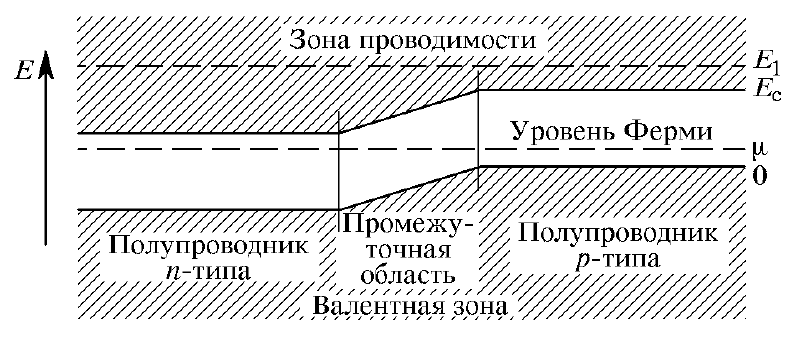
\includegraphics[width=0.4\textwidth]{energy_scheme.png}
		\caption{Энергетическая схема $(p-n)$-перехода, находящегося в равновесии}
		\label{pic:energy_scheme}
	\end{figure}  
	
	На рисунке \ref{pic:energy_scheme} $E_c$ обозначена энергия, соответствующая дну зоны проводимости, $\mu$ --- уровень Ферми. В этих обозначениях при обычных температурах концентрация электронов $n_n$ в зоне проводиомсти и концентрация дырок $n_p$ в валентной зоне равны соответственно: 
	
	\[ n_n(n\text{-область}) = Q_n\exp\left(-\frac{E_c - \mu}{kT}\right) \]
	
	\[ n_p(p\text{-область}) = Q_p\exp\left(-\frac{\mu}{kT}\right) \]
	
	Из-за наличия контактной разности потенциалов $\Delta V$ между концентрациями основных и неосновных носителей тока в области устанавливается следующее соотношение:
	
	\[ \frac{n_n(n\text{-область})}{n_n(p\text{-область})} = \frac{n_p(p\text{-область})}{n_p(n\text{-область})} = \exp{\left(\frac{e\Delta V}{kT}\right)} \]
	
	Здесь индекс по-прежнему указывает на тип носителя, а в скобках стоит рассматриваемая область полупроводника.
	
	Проходящий через переход ток $I_0$ пропорционален концентрации неосновного заряда в области: 
	
	\[ I_0 \propto n_n(p\text{-область}) = n_n(n\text{-область}) \cdot \exp{\left(-\frac{e\Delta V}{kT}\right)} \]
	
	Приложим теперь к $(p-n)$-переходу напряжение $V_\text{ист}$ от внешнего источника, чтобы $p$-область заряжалась положительно относительно $n$-области (см. рисунок \ref{pic:external_voltage}.a). Потенциальный барьер снижается в $\exp{\left(\frac{eV_\text{ист}}{kT}\right)}$ раз, и ток, протекающий через переход слева направо, увеличивается в соответствующее количество раз. Ток справо налево остается неизменным и равен $I_0$. Тогда полный ток $I$ через барьер равен разности токов, текущих направо и налево: 
	
	\[ I = I_0\left(\exp\left(\frac{eV_\text{ист}}{kT}\right) - 1\right) \]
	
	Аналогичное равенство справедливо и для тока, переносимого дырками. 
	
	При приложении обратного напряжения (см. рисунок \ref{pic:external_voltage}.б)) полный ток также описывается формулой, данной выше.
	
	\begin{figure}[h]
		\centering	
		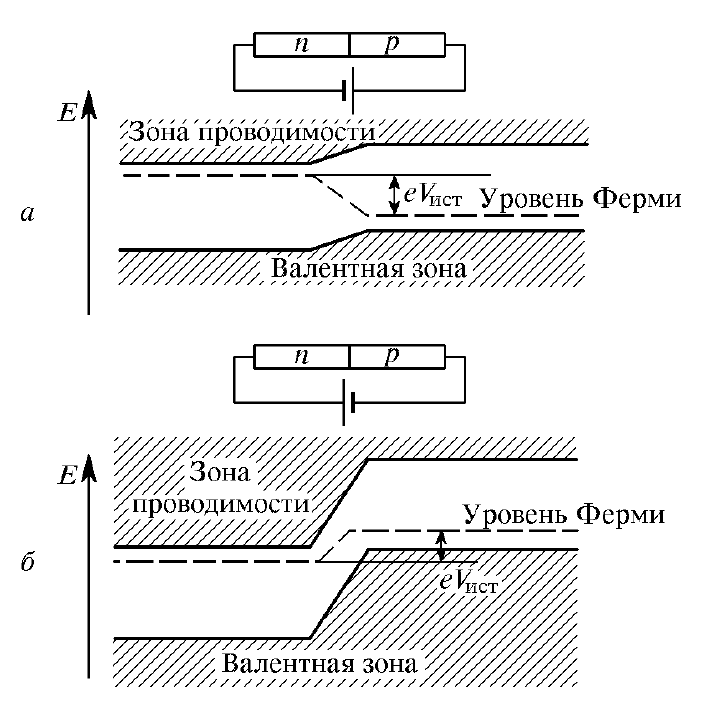
\includegraphics[width=0.4\textwidth]{external_voltage.png}
		\caption{Схема $(p-n)$-перехода под внешним напряжением с положительным (а) и отрицательным (б) смещениями области перехода}
		\label{pic:external_voltage}
	\end{figure} 
	
	Таким образом, при приложенном внешнем напряжении $V_\text{ист}$ суммарный ток электронов и дырок равен: 
	
	\[ I = (I_{0, n} + I_{0, p}) \left(\exp\left(\frac{eV_\text{ист}}{kT}\right) - 1\right) = A(n_n(n\text{-область}) + n_p(p\text{-область})) \cdot \exp\left(-\frac{e\Delta V}{kT}\right)\left(\exp{\left(\frac{eV_\text{ист}}{kT}\right)} - 1\right) = \]
	
	\[ = C \exp\left(-\frac{e\Delta V}{kT}\right)\left(\exp{\left(\frac{eV_\text{ист}}{kT}\right)} - 1\right) \]
	
	В последнем равенстве учтено, что концентрации электронов и дырок определяются концентрацией примесей и мало зависят от температуры. 
	
	При комнатных температурах справедливо приближение: $eV_\text{ист} \ll kT$. Тогда для полного тока через переход верно: 
	
	\[ I = C\exp{\left(-\frac{e\Delta V}{kT}\right)} \cdot \frac{eV_\text{ист}}{kT} \]
	
	Из полученного выражение для тока $I$ найдем сопротивление $R$ $(p-n)$-перехода: 
	
	\[ R = \frac{V_\text{ист}}{I} = \frac{1}{C} \cdot \frac{kT}{e} \exp{\left(\frac{e\Delta V}{kT}\right)} \propto \exp{\left(\frac{e\Delta V}{kT}\right)}\]
	
	При написании последнего равенства мы пренебрегли слабой зависимостью от температуры предэкспоненциального члена, которая
	мало заметна на фоне быстрой экспоненциальной зависимости.
	
	Логарифмируя и дифференцируя последнее выражение, получим искомую формулу для нахождения контактной разности потенциалов:
	
	\begin{equation}\label{dV}
	\Delta V = \frac{k}{e}\cdot \frac{\Delta(\ln R)}{\Delta(1/T)}
	\end{equation}
	
		\section{Экспериментальная установка}
	
	Схема установки для измерения температурной зависимости контактной разности потенциалов $\Delta V(T)$ показана на рисунке \ref{pic:scheme}. Она состоит из мостиковой схемы и термостата. Источником питания схемы служит генератор прямоугольных импульсов, а сигнал с балансируемого моста подается на независимые каналы осциллографа. 
	
		\begin{figure}[h]
		\centering	
		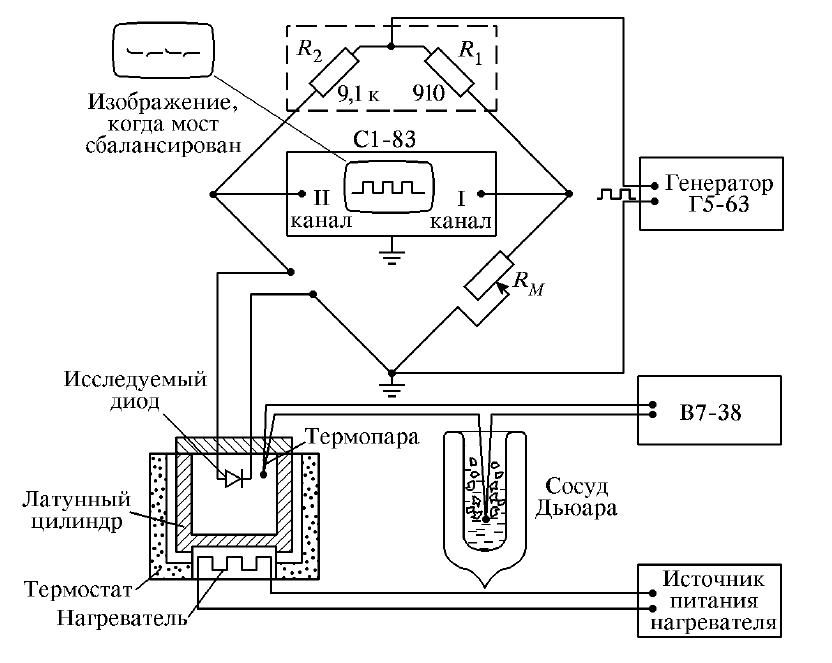
\includegraphics[width=0.4\textwidth]{scheme.png}
		\caption{Экспериментальная установка для определения контактной разности потенциалов $(p-n)$-перехода}
		\label{pic:scheme}
	\end{figure} 

	
	На схеме на рисунке \ref{pic:scheme} указаны также номиналы используемых резисторов. Сопротивление диода $R$ выражается через сопротивление магазина $R_M$ и сопротивления $R_1 = 910$ Ом, $R_2 = 9.1$ кОм:
	
	\[ R = \frac{R_2}{R_1}R_M = 10\cdot R_M \] 
	
	\section{Выполнение работы}
	
	Измерения проводятся в интервале температур от комнатной до $\approx 80^o$C. Температура образца измеряется медно-константановой термопарой, постоянная которой равна $\alpha = 41$ мкВ/K.
	
	До включения цепи температура образца совадала с комнатной  ($T_0 = 298$ К), сопротивление на концах термопары при этой было равно $\Delta U_{0} = 0,06$ мВ.
	
	Снимем зависимость сопротивления магазина $R_M$ при сбалансированном мосте от напряжения на термопаре $\Delta U$. По $R_M$ пересчитаем сопротивление диода $R = 10R_M$. Зная константу термопары $\alpha$,  получим температуру образца $T$ для соответствующего измерения напряжения: 
	
	\[ T = T_0 + \frac{\Delta U - \Delta U_{0}}{\alpha} \] 
	
	Измерения и последующие вычисления содержатся в таблице \ref{table_5}. Погрешность показаний вольтметра примем равной $ 0,01 $ мВ; относительная погрешность сопротивления магазина, в соответствии с указанием на приборе, составит 5\%. Первое измерение сделано при выключенной печи. 
	
		\begin{table}[h]
		\caption{Результаты измерений}
		\begin{center}
			\begin{tabular}{|c|c|c|c|c|c|c|c|c|}
				\hline
				№ & $ \Delta U  $, мВ & $ R_м $, Ом &  $ T $, K & $ \dfrac{1}{T}, \; 10^{-3} \; К^{-1} $ & $ \sigma_{\frac{1}{T}}, \; 10^{-3} \; К^{-1}  $ &  $ R $, кОм & $ \sigma_R $, кОм &  $ \ln \left( \dfrac{R}{R_m} \right)  $ \\
				\hline
			1 & 0.06 & 331 & 298 & 3.356 & 0.017 & 3.31 & 0.17 & 3.72 \\
			2 & 0.265 & 213 & 303 & 3.3 & 0.016 & 2.13 & 0.11 & 3.28 \\
			3 & 0.47 & 135 & 308 & 3.247 & 0.016 & 1.35 & 0.07 & 2.83 \\
			4 & 0.675 & 91 & 313 & 3.195 & 0.015 & 0.91 & 0.05 & 2.43 \\
			5 & 0.88 & 64 & 318 & 3.145 & 0.015 & 0.64 & 0.03 & 2.08 \\
			6 & 1.085 & 48 & 323 & 3.096 & 0.014 & 0.48 & 0.02 & 1.79 \\
			7 & 1.29 & 35 & 328 & 3.049 & 0.014 & 0.35 & 0.02 & 1.48 \\
			8 & 1.495 & 28 & 333 & 3.003 & 0.014 & 0.28 & 0.01 & 1.25 \\
			9 & 1.7 & 21 & 338 & 2.959 & 0.013 & 0.21 & 0.01 & 0.97 \\
			10 & 1.905 & 16 & 343 & 2.915 & 0.013 & 0.16 & 0.01 & 0.69 \\
			11 & 2.11 & 13 & 348 & 2.874 & 0.012 & 0.13 & 0.01 & 0.49 \\
			12 & 2.315 & 11 & 353 & 2.833 & 0.012 & 0.11 & 0.01 & 0.32 \\
			13 & 2.52 & 8 & 358 & 2.793 & 0.012 & 0.08 & 0 & 0 \\
			\hline
			\end{tabular}
		\end{center}
		\label{table_5}
	\end{table}

	Погрешность температуры $T$ будем считать равной 1,5 К для всех измерений, погрешность величины $ \sigma_{\ln \left( \frac{R}{R_m} \right)} \approx 0,07 $ для всех измерений. Построим график зависимости $ \ln \left( \dfrac{R}{R_m} \right)  $ от обратной температуры $ \dfrac{1}{T} $.
	
	\begin{figure}[h]
		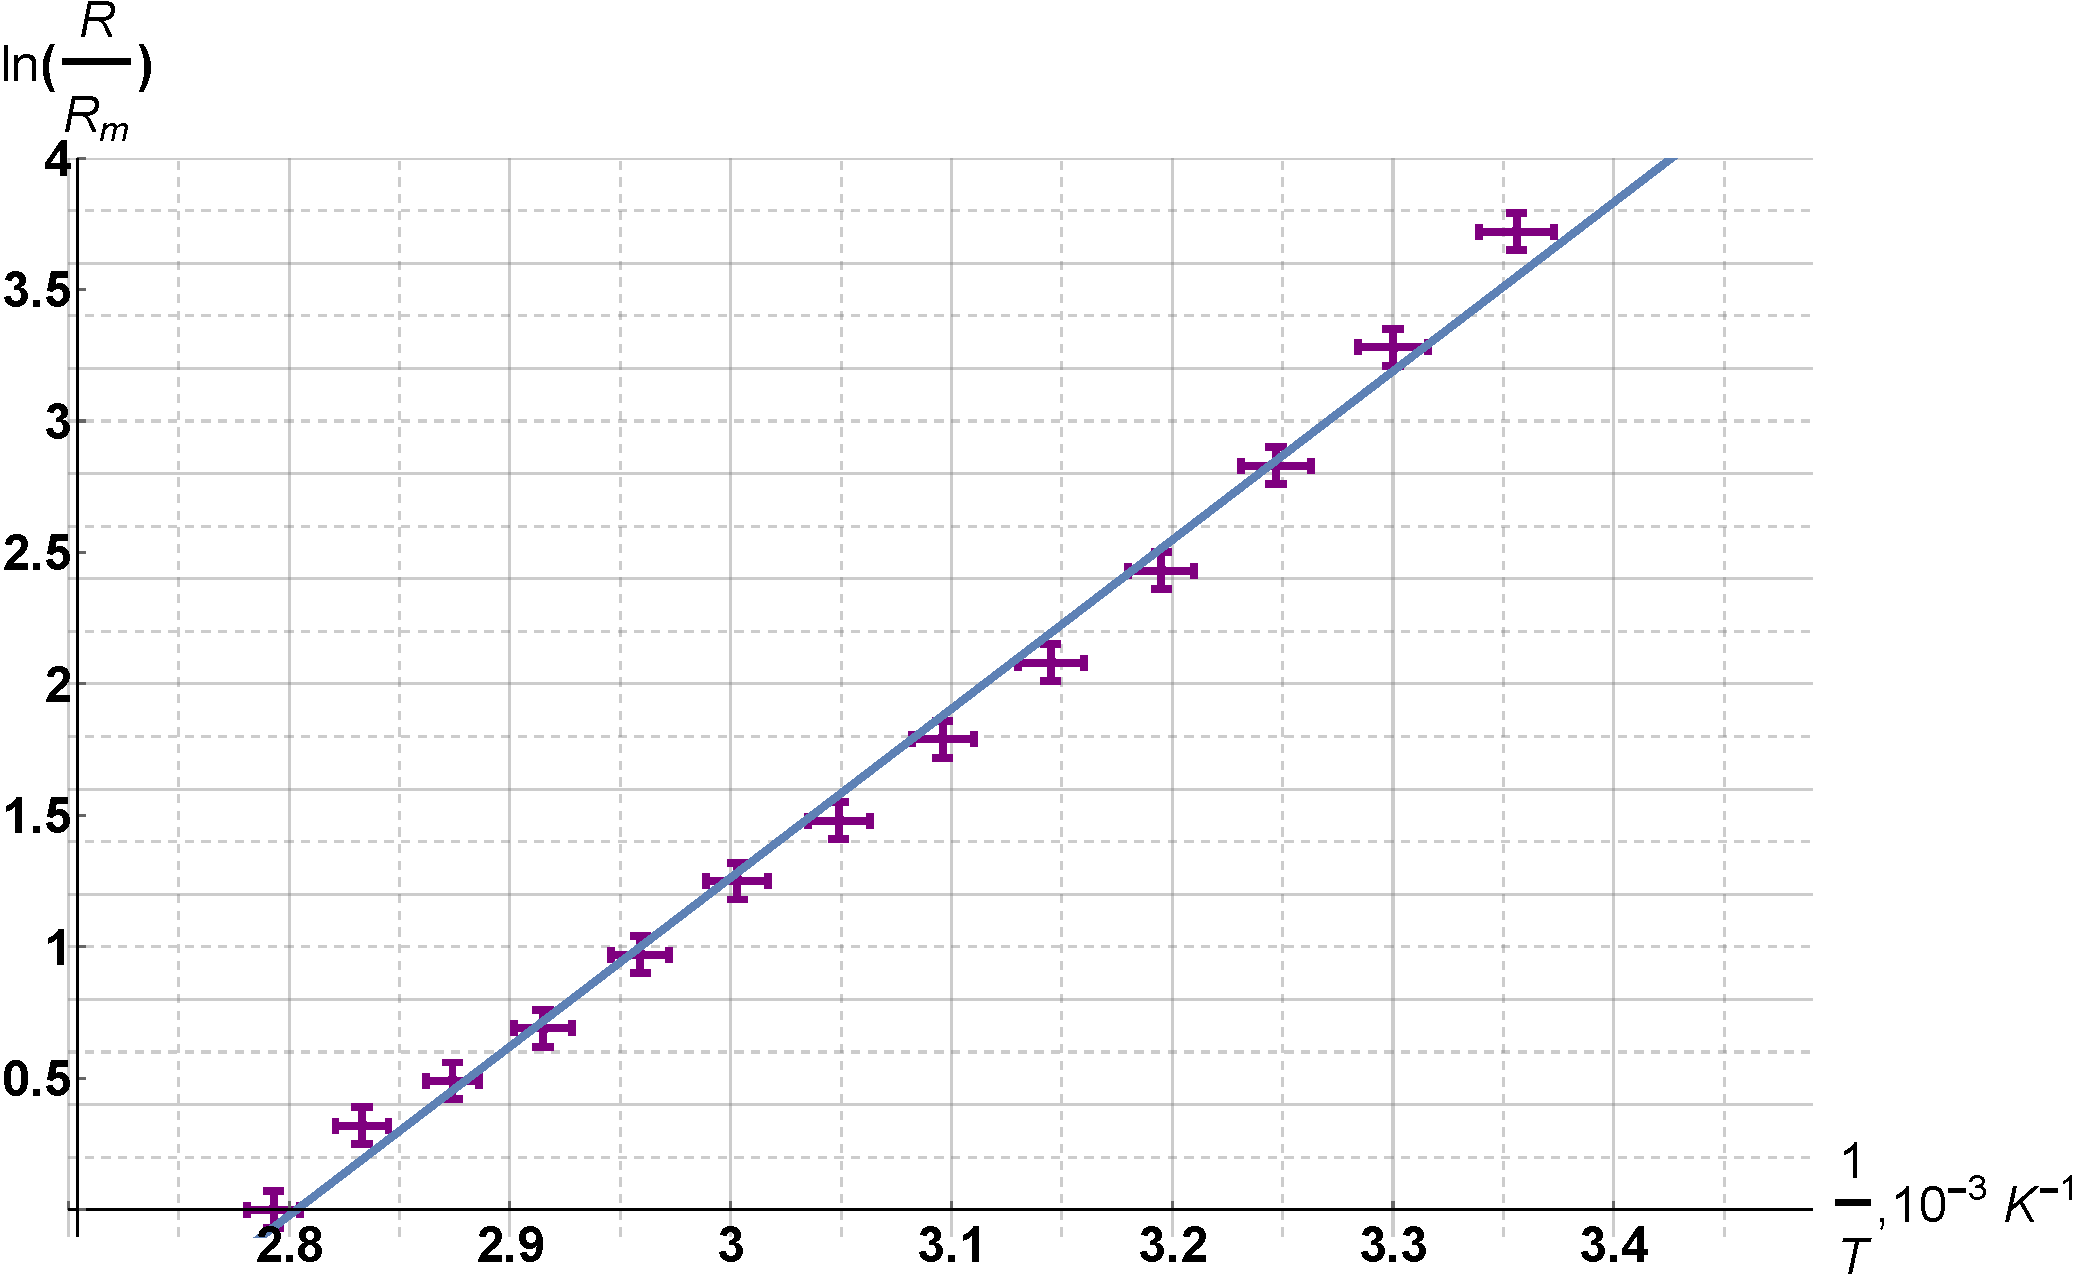
\includegraphics[scale=0.47]{graf.pdf}
		\caption{График зависимости $ \ln \left( \dfrac{R}{R_m} \right) $ от $ \dfrac{1}{T} $}
		\label{graf}
	\end{figure}

\begin{table}[H]
	\caption{Фит рис. \ref{graf} функцией $ y = ax + b $}
	\begin{center}
		\begin{tabular}{|c|c|c|}
			\hline
			& \text{Estimate} & \text{Standard Error} \\
			\hline
			$ b $ & -18.004 & 0.464\\
			$ a $ & 6.42& 0.15 \\
			\hline 
		\end{tabular} 
	\end{center}
	\label{}
\end{table}
	
	Получив из параметров фита коэффициент наклона фита $ a' = 10^3 \x a \; К \approx (6,42 \pm 0,15 ) \x 10^3 \; К $, из формулы \eqref{dV} находим искомую контакную разность потенциалов $ (p -- n) $-перехода полупроводникового диода:
	
	\begin{equation}\label{}
	\Delta V = \dfrac{k}{e} \x a' \approx 0,554 \pm 0,013 \; В
	\end{equation}
	
	
	\section{Вывод }
	
	Таким образом, в этой работе мы измерили температурную зависимость сопротивления полупроводникового диода. Она оказалась совпадающей с теорией. По этой зависимости определена контактная разность потенциалов $(p-n)$-перехода. 
	
\end{document}
